\scanpage{15}
\inserted{(Condition différentielle)}
d) Tout $\mathcal A_n$ est stable par les op. différentiels élémentaires $D_{\unsure{n|\underline n}}$ [$\Longrightarrow$ si $f(x_1,\ldots,x_n,y_1,\ldots,y_m)\in \mathcal A_{n+m}$ est mis sous la forme $\sum_{p\in\mathbb N^m}f_p(x)y^p$, alors les $f_p$ sont $\in \mathcal A_n$]
\margin{en car. 0 c'est équivalent à la stabilité par les $\frac{\partial}{\partial x_i}$.}
\figure{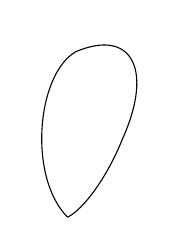
\begin{tikzpicture}\draw (0,0)..controls(-.5,.5)and(-.4,1.8)..(.1,2.1)..controls(.8,2.4)and(1.1,1.9)..(.7,1)..controls(.5,.5)and(.2,.1)..(0,0);\end{tikzpicture}}

Ceci implique que les algèbres $P^n_{X/k}$ sur $\mathcal O(X)$ ($X$ un \deleted{$\mathcal A_*$} schéma $\mathcal A_*$-formel) ont \deleted{une} $\mathcal A_*$ structure canonique et fonctorielle, de $=$ $P^n_{X/Y}$ si $X\to Y$ est un $\mathcal A_*$-morphisme submersif, de $=$ \deleted{\unsure{pour}} si $X\supset Y$ est un couple de schémas $\mathcal A_*$-formels, $\mathcal O(Y)=\mathcal O(X)/J$, les \unsure{voisinages normaux|voisinages infinitésimaux} $\mathcal O_X/J^n$ ont des $\mathcal A_*$-structures canoniques, fonctorielles, compatibles aux images inverses transversales. L'op. diff. universel d'ordre $n$
\[
\mathcal O(X)\mathbin{-}P^n_{X/k}
\]
\deleted{\unsure{est un} $\mathcal A_*$ morphisme} applique $\mathcal O_{\mathcal A_*}(X)$ dans $(P^n_{X/k})_{\mathcal A_*}$ \deleted{$\unsure{\mathcal O_{\mathcal A_*}}$} $\ldots\ldots$

\deleted{\unsure{Et}} Les $\operatorname{Diff}_n(X/k)$ (duals des $P^n_{X/k}$) ont \deleted{\unsure{une}} $\mathcal A_*$-structures canoniques, leur composition \deleted{est} laisse stables les parties $\operatorname{Diff}_n(X_{\mathcal A_*}/k)$ des $\mathcal A_*$-op. diff., et ces derniers stabilisent les \deleted{$\unsure{\mathcal A_*}$} $\mathcal O_{\mathcal A_*}(X)\ldots\ldots$ Idem pour les op. diff. relatifs, pour $X\to Y$ $\mathcal A_*$-morphisme \deleted{\unsure{étale}} \inserted{submersif}.

\uline{Cor} $\mathcal A_n\subset k_0[[t_1,\ldots,t_n]]$. \deleted{\unsure{Les coefficients étant dans} $k_0$} D'où un foncteur $\unsure{M\mathbin{\bullet}\to|M_{\mathcal A_*}}$ des schémas $\mathcal A_*$-formels vers les schémas formels sur $k_0\ldots$
\deleted{Soit $X\longrightarrow Y$ un morphisme submersif de schémas formels, sur $X$}
\figure{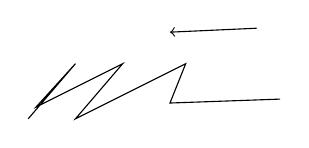
\begin{tikzpicture}[x=1cm,y=1cm]\draw (0,0)--(.6,.7)--(.1,.15)--(1.2,.7)--(.6,0)--(2,.7)--(1.8,.2)--(3.2,.25);\draw[<-] (1.8,1.1)--(2.9,1.15);\end{tikzpicture}}
\mspage{14}
